Researchers found that advances in the field of deep learning -- a broad family of methods based on artificial neural networks -- can be used to enhance the classical RL algorithms.
This led to the expansion of the field, marking the birth of \textbf{deep reinforcement learning (deep RL)}.

Classic RL assumes that the state space is finite and can be modeled in a tabular manner.
However, we seldom encounter real-world, interesting problems where this assumption holds.
Deep RL is an open field striving to solve \emph{more complex} problems than classical methods allow.
This is done through the ability of functional approximators to model high-dimensional spaces.

The field has recently surged, after a series of new algorithms and succesful applications were published.
In this chapter, we try to give an overview of the main methods of learning but mainly focus on developing \emph{Mnih et al.'s \textbf{DQN} (2013)} \cite{atari-dqn}.

In Section \ref{section:convnets}, we present \textbf{convolutional neural networks}, a class of artificial neural networks which became the foundation of multiple algorithms in deep RL.

Section \ref{section:dqn} covers using neural networks (called deep Q-networks in the paper \cite{atari-dqn}) as approximators in Q-learning in order to build autonomous agents for complex model-free environments.

The rest of the chapter (Sections \ref{section:pg} and \ref{section:actor-critic}) deals with alternative strategies for doing (deep) model-free control, namely \textbf{policy optimization} and \textbf{actor-critic} methods respectively.

\clearpage

\subsection{Convolutional Neural Networks (ConvNets)} \label{section:convnets}
\textbf{Convolutional neural networks} (often shortened as ConvNets or CNNs) are a specific type of artificial neural network for processing data that has a known grid-like topology \cite{Goodfellow-et-al-2016}.

ConvNets exploit the \textbf{spatial nature} of the data.
This property makes them especially useful over a vast spectrum of problems, such as image classification, audio signal processing, analyzing financial time-series etc.
Among those, image classification tasks are the primary reason for the architecture's popularity.

The \textbf{origin} of convolutional networks can be traced back to Kunihiko Fukushima's \emph{neocognitron} (1979).
Kunihiko’s design \cite{neocognitron-paper} was itself inspired by earlier breakthroughs in neuroscience -- namely studies of the visual cortex of mammals (Hubel \& Wiesel, 1959).
LeCun et al. (1989) further improved this model by introducting backpropagation training, which set the standard for today’s architectures.

\subsubsection{Overview}
A convolutional network contains at least one convolutional layer in its structure.
A typical convolutional layer (represented in Figure \ref{fig:conv-layer}) is composed of three stages \cite{Goodfellow-et-al-2016}:
\begin{enumerate}
    \item The \textbf{convolution stage} convolves the input data with a filter (kernel), which results in a set of linear activations.
    The kernel is the learned element, i.e. we learn the weights of the kernel as we would learn the weights of a linear layer.
    \item The \textbf{detector stage} pipes each linear activation from the convolution layer thorugh a non-linear activation function (e.g. ReLU \footnotemark)
    \item The \textbf{pooling stage} is an optional stage which reduces the output size by computing summary statistics over the data.
\end{enumerate}
\footnotetext{standing for \emph{rectified linear unit}, it is commonly used as an activation function in neural networks. In its classic form, it can be expressed as $f(x) = max(0, x)$.}

\begin{figure}[h]
    \centering
    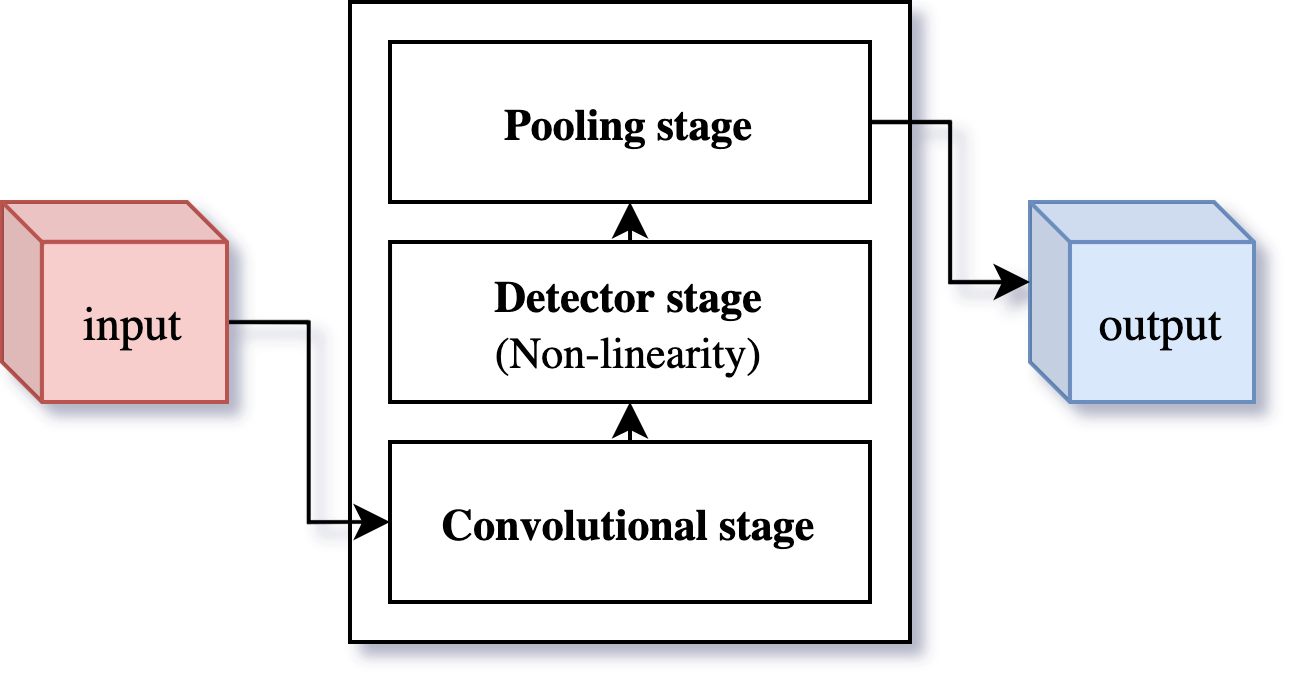
\includegraphics[width=0.7\textwidth]{conv-layer-structure.png}
    \caption{A schematic of a convolutional layer.}
    \label{fig:conv-layer}
\end{figure}

In this section, we consider the \textbf{input} and \textbf{output data} to be 3D tensors, consisting of a spatial dimension (width and height) and a depth dimension.
Visualizing this process with images in mind is particularly helpful to understanding.
The spatial dimensions map exactly to the width and height of an image, and each color channel can be considered a separate depth level.


\subsubsection{The Convolutional Stage}
This stage performs the convolution operation which is the most computationally demanding procedure of the layer.
The output from this stage is a \textbf{feature map} of the input, which is then passed as linear activation to the detector stage, likewise to fully-connected feedforward networks.

This \textbf{operation} consists of sliding a \emph{kernel} over the input.
At every step, we compute the dot product between the kernel and the volume of input it currently overlaps.
The \textbf{kernel} (or filter) is a tensor of adjustable weights, which is small relative to the image's spatial dimentions but must cover the entire depth of the image.
The effects of the convolutional stage are determined by a number of hyperparameters: depth, stride and padding.

A convolutional stage can learn multiple independent kernels.
The number of kernels is given by the \textbf{depth} hyperparameter.
It is conveniently called such because it corresponds to the depth of the output of this stage.
A \textbf{depth column} (or fibre) \cite{stanford-convnets} is a set of neurons ``looking'' to the same region in the input (where each neuron corresponds to a different kernel) .

The \textbf{stride} specifies the distance which we slide the kernel with over the input at each step.
Some models provide separate stride parameters for each axis (horizontal and vertical) \cite{Goodfellow-et-al-2016}.

\textbf{Zero-padding} (or simply padding) enables padding our input data with zeros along the borders. It is useful for controlling output size, especially in cases where we want to preserve the input size over multiple layers.

\begin{figure}[h]
    \centering
    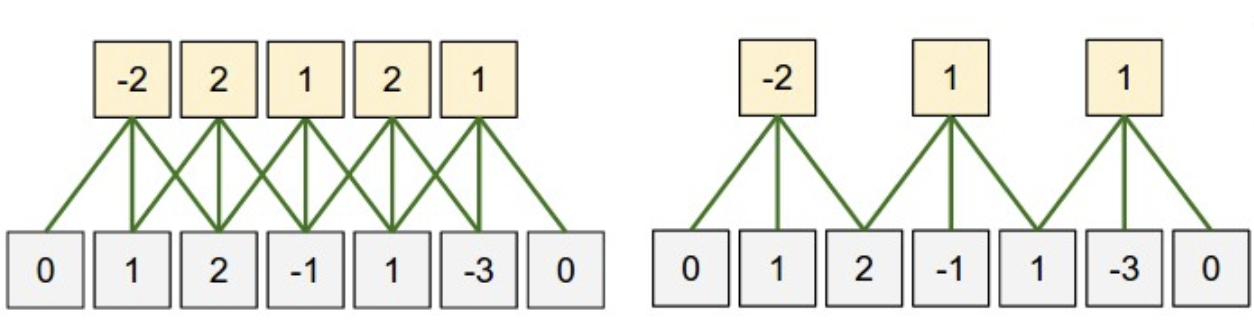
\includegraphics[width=0.6\textwidth]{conv-stride-padding.png}
    \caption{(Left) Using a stride of 1 and a zero-padding of 1 to preserve the original spatial dimensions of the input. (Right) Using a padding of 1 and a stride of 2, which results in fewer output values. (Illustration from \cite{stanford-convnets})}
    \label{fig:conv-stride-padding}
\end{figure}
 
The properties of convolution confer ConvNets a myriad of advantages over fully-connected feedforward neural networks.
This gain in efficiency comes from the assumption that the data has an underlying spatial structure, which can be exploited better by ConvNets than by alternatives.

Typical fully-connected layers relate all their outputs to all their inputs by separate, \emph{independently adjustable} weights.
This requires storing weight matrices as large as the input data itself, rising the computational cost as input size grows.
In contrast, kernels are significantly smaller than the input volume is (in the spatial dimensions).
Kernels are also reused across the entire layer (\textbf{parameter sharing}), resulting in smaller memory requirements.

ConvNets feature \textbf{sparse interactions}, in contrast to the dense interactions of fully-connected layers in which every output is related by a weight to each of the input values.
This boosts learning efficiency by reducing the number of necessary computations.

Learning smaller, shared kernels can be a means of controlling \emph{overfitting} \cite{Goodfellow-et-al-2016}. Moreover, ConvNets can operate on input data of \textbf{varying sizes} without making adjustments to model architecture.


\subsubsection{Pooling}
The \textbf{pooling stage} is an optional stage in the ConvNet architecture which performs a \emph{downsampling} of its inputs.
The role of this stage is to gradually reduce computation (and memory requirements) in the network by reducing the spatial dimension of the data \cite{stanford-convnets}.
It processes output from the convolutional stage by applying a pooling function.

A \textbf{pooling function} computes a summary statistic (e.g. maximum, average, $l^2$-norm etc.) over a neighbourhood of input values \cite{Goodfellow-et-al-2016}.
The pooling stage has a similar operation to the convolutional stage:
a moving window is slided over and across the input data and at each step, the summary is computed.

Each depth slice of the data is processed independently.
An example for a simple but commonly used operation (max pooling) is shown in Figure \ref{fig:maxpooling}.

\begin{figure}[h]
    \centering
    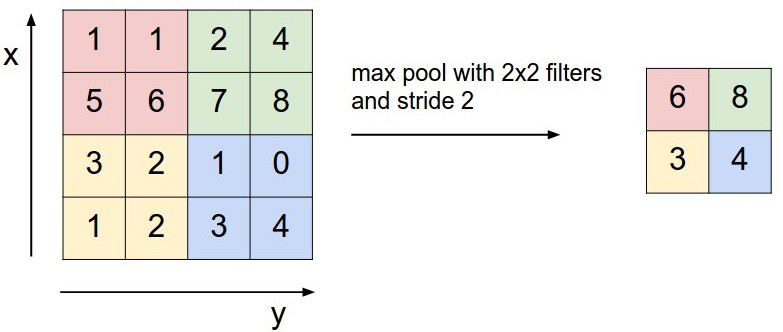
\includegraphics[width=0.8\textwidth]{conv-maxpooling.jpg}
    \caption{Simple example illustrating max pooling (on a single depth level). Illustration from \cite{stanford-convnets}.}
    \label{fig:maxpooling}
\end{figure}

\subsection{Deep Q-Networks (DQN)} \label{section:dqn}
To reiterate our chapter introduction, a key challenge of applying RL to real-world problems is data representation (in the form of policies and value functions).
Real applications require modelling large, high-dimensional problem spaces and hence depend upon functional approximation.

Most succesful systems (prior to DQN) have relied on \textbf{handcrafted feature sets}, created by experts to capture the problem-relevant information so the RL system does not have to.
A \textbf{feature} is an independent, measurable property of an observed phenomenon.
Choosing which features of the training data yield the most \emph{relevant} information (and subsequenlty lead to more effective learning) is a central problem in machine learning.

Other attempts have relied on \textbf{autoencoders}\footnotemark{} as a preprocessing step, to lower the dimensionality of observations before feeding them to the RL agent (used for example in neural fitted Q-iteration \cite{neural-q-fitted}).
\footnotetext{neural networks capable of learning an efficient representation of the data in an unsupervised manner.}

This section introduces \emph{Mnih et al.}'s \textbf{DQN} \cite{atari-dqn}, a deep model-free learning method that uses \textbf{automatic feature extraction} (i.e., is capable of finding an efficient representation directly from interactions with the environment).

The paper benchmarks its approach on 49 video games for the Atari 2600, using the Atari Learning Environment (ALE) \cite{ale-paper} -- an extension on top of an Atari emulator, designed to transform \emph{games} into \emph{task environments}.
The selection features diverse mechanics, with some games requiring agents to develop long-term strategies to perform reasonably well at.

The researchers trained agents separately for each game using the same architecture and hyperparameters.
Each agent would start with \emph{randomized weights} and would learn relying exclusively on raw video input and reward signals ($1$ for a score increase, $-1$ for a score decrease, or $0$ otherwise) from the ALE.

The approach was demonstrated to perform well in widely different environments, with no prior knowledge of any of them.

DQN scored better than existing methods (including NEAT\footnotemark) on the vast majority of the games.
\footnotetext{standing for \emph{neuroevolution of augmenting topologies}, a genetic algorithm for generating neural network topologies.}
It managed \emph{human-like} performance at a significant number of games, according to the evaluation techniques used in the paper.
The agent scored highest in \emph{Pong}, \emph{Enduro} and \emph{Breakout}, outperforming expert human players \cite{atari-dqn}.

\subsubsection{Overview}
The algorithm described in the paper is roughly based on \textbf{Q-learning} (described in Section \ref{rl:q-learning}), fitted with deep convolutional networks which approximate the action-value function $Q$, suggestively called \textbf{deep Q-networks}.

The learning rule is formulated in (\ref{eqn:deepq-learning-rule}) and represents a \emph{semi-gradient version} of the Q-learning update in (\ref{eqn:q-learning-update-rule}).
The values of a state-action pair $(s, a)$ are obtained by performing a forward pass through a Q-network, which we denote by $\hat{Q}(s, a; \theta)$, where $\theta$ represents the weights of the network.

\begin{equation} \label{eqn:deepq-learning-rule}
    \theta_{i + 1} = \theta_{i} + \alpha [
        R_{t+1}
        + \gamma \max_{a \in A}{\hat{Q}(S_{t+1}, a; \theta_{i})}
        - \hat{Q}(S_{t}, a; \theta_{i})
    ]
    \nabla{\hat{Q}(S_t, A_t, \theta_{i})}
\end{equation}

The gradient in (\ref{eqn:deepq-learning-rule}) is computed by backpropagation and uses \emph{mini-batch gradient descent} in conjunction with the \emph{RMSProp} algorithm \cite{atari-dqn}.

\textbf{Mini-batch gradient descent} is a variation of gradient descent (GD) which computes the error for a relatively small subsequence of examples from the training dataset.
This has the advantage of being more computationally efficient than stochastic GD (which performs the calculation for only one example), while avoiding to load the entire batch into memory (as in full-batch GD).

\textbf{RMSProp} is a gradient descent algorithm proposed by Geoff Hinton in 2012.
The idea behind it is that the network can achieve faster convergence by adjusing a separate step-size for each weight.
Each step-size is fine-tuned based on a \emph{moving average} of the (most recent) gradient magnitudes of its corresponding weight.

% This should remain the end paragaph, in order to transition to explanations for experience replay and target networks.
Off-policy learning, bootstrapping (both characteristics of Q-learning) and functional approximation are \textbf{incompatible} at a fundamental level (the three elements comprise the so-called \emph{deadly triad} \cite{rlai}), as the combination fails to converge in theory.
In order to work properly, DQN modifies Q-learning in a few fundamental ways to overcome this incompatibility, by using \textbf{experience replay} and an additional \textbf{target network}.

\subsubsection{Experience Replay}

A \textbf{transition} (or episode) is a tuple $e_t = (S_t, A_t, R_{t+1}, S_{t+1})$, consisting of the initial state-action pair at time-step $t$, along with the reward and the successor state.
\textbf{Experience replay} consists of accumulating the agent's experienced transitions over multiple episodes of play in a \emph{replay memory} $\mathcal{D}$.

At every step of learning, the algorithm samples from the replay memory to generate a \textbf{mini-batch} of transitions.
In this variant of Q-learning, the successor state is no longer the direct successor $S_{t+1}$, but instead is an entirely disconnected experience, chosen at random from $\mathcal{D}$.
Being off-policy, Q-learning is resilient to this adjustment and thankfully still adheres to its classical properties \cite{rlai}.

Storing experiences over time allows for better \emph{sample efficiency} by reusing previous experiences over multiple update steps.
The \emph{random sampling} aspect plays a key role in DQN by decoupling highly correlated states.
This, in effect, reduces variance by removing the dependence of succesive experiences on the network's weights at that point \cite{rlai}.

\subsubsection{Target Network}

In vanilla Q-learning, the learning rule evaluates two successive states under the \emph{same} action-value function.
However, when using a neural network to approximate the action-value function, this creates an unnecessary dependency of the network's weights $\theta_{i+1}$ on the previous set of weights $\theta_{i}$.
In the usual setting of supervised learning, neural networks are optimized to learn fixed, well-defined labels.
By contrast, our learning rule in (\ref{eqn:deepq-learning-rule}) enforces a ``moving target’’ which can lead to \textbf{divergence}.

To counteract this, DQN introduces a \textbf{target network}, with an identical architecture to the main Q-network. This network stores the weights of the main network ``frozen'' at some previous point during training.
In this way, we provide a \emph{fixed target} for our main network to ``move'' towards.
Finally, in order to make progress, the networks need to be periodically swapped.
The swap frequency is specified by a hyperparameter.

% Conclusion?
% The algorithm as given in the paper to tie it all up?
% Sprinkle some images?

\subsection{Policy Gradients} \label{section:pg}

The DQN method presented in the previous section applies methods from supervised learning in order to approximate a value function. Because of this, the algorithm is a type of \emph{value function approximation}.
We learn a representation of our value function by adjusting a set of parameters $\theta$ which represent the weights and biases of a neural network.
\begin{equation}
    Q(s, a) \approx \hat{Q}(s, a; \theta)
\end{equation}

In constrast, \textbf{policy-based reinforcement learning} directly paramerizes the \emph{policy}.
\begin{equation}
    \pi(a \given s) \approx \hat{\pi}(a \given s; \theta) \mbox{ also denoted as } \pi_{\theta}(a \given s)
\end{equation}

This has a series of advantages over value approximation methods.
For example, it has \textbf{better convergence} properties as the problem it solves is -- in some sense -- less complex.
Value-based methods are trying to approximate the exact score that a state might yield, which is a relatively complicated task.
By contrast, a learned policy only needs to have a proper distribution over the actions to perform well, without making any assumption about the actual values.

Policy-based methods also have an advantage with \textbf{continuous action spaces}.
Continuous action spaces are especially important for robotics, where we often represent movement using rotation and force vectors.
The $max$ operator in Q-learning and Sarsa does not scale to continuous spaces, making them unsuitable for certain types of tasks (at least without significant extensions and tweaking).

A key advantage of policy-based learning is being able to directly learn the \textbf{optimal stochastic policy}.
In the classical (tabular) case, we assumed perfect state representation -- hence, a deterministic policy would indeed be the optimal policy.
However, in the approximated case, deterministic policies can fail due to partial observability of the environment (since we are relying on \emph{features} which by definition are relevant but partial information).

A feature set might be insufficient to distinguish some states from others. This phenomenon is referred to as \textbf{state aliasing}.
Consider a situation in which we cannot distinguish between two grey tiles, as shown in the gridworld in Figure \ref{fig:state-aliasing}.
A deterministic agent could decide to go either East or West on \emph{both} grey tiles.
Either choice results in a possibility of getting stuck (the policy creates a loop).
A stochastic policy assigning $0.5$ to both East and West on a grey tile would perform better in this case.

\begin{figure}[h]
    \centering
    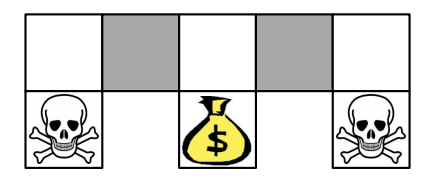
\includegraphics[width=0.3\textwidth]{silver-state-aliasing.png}
    \caption{An aliased gridworld. (Illustration from \cite{silver-lectures})}
    \label{fig:state-aliasing}
\end{figure}

The premise of policy optimization is the existence of an \textbf{objective function} $J(\theta)$ measuring the quality of $\pi_{\theta}$.
The problem of optimizing $J$ is solvable by a vast array of techniques such as hill climbing, simulated annealing etc.

One effective way to maximize the objective function is by \textbf{gradient ascent}, which is the foundation of this class of algorithms.
For this, we move our current set of weights \emph{slightly} (i.e., the extent is given a step-size $\alpha$) towards the direction given by the gradient of the performance measure $J(\theta_{t})$ with regard to its argument.
\begin{equation} \label{eqn:pg-general-rule}
    \theta_{t+1} \leftarrow \theta_{t} + \alpha \hat{ \nabla_{\theta_{t}} J(\theta_{t}) }
\end{equation}

Methods which follow this schema, regardless of whether or not they use an additional value function, are considered \textbf{policy gradient methods} \cite{rlai}.

The performance of a policy generally depends on $\theta$ in two ways:
\begin{itemize}
    \item It \emph{directly} depends on how $\pi_{\theta}$ selects actions.
    \item It \emph{indirectly} depends on the distribution of the states in which those actions are taken.
\end{itemize}
Considered independently, action selection's influence on $\theta$ can be clearly observed.
Given a state $s$, the direct effect of $\theta$ on actions can be observed directly by looking at obtained rewards.
In the latter case, the effect our policy has on the state distribution depends on the environment and is generally \emph{unknown} \cite{rlai}.

The \textbf{policy gradient theorem} (PCT) provides an expression for the gradient of the performance with regard to its arguments which does not depend on the state distribution \cite{rlai}.
The expression is given in (\ref{eqn:pg-theorem}) for the episodic case.
\begin{equation} \label{eqn:pg-theorem}
    \nabla_{\theta} J(\theta) \propto
        \sum_{s}{
            \mu(s) \sum_{a}{
                q_{\pi_{\theta}}(s, a) \nabla_{\theta} \pi_{\theta}(a \given s)
            }
        }
\end{equation}

\subsubsection{Monte Carlo Policy Gradients}
\textbf{Monte Carlo policy gradients} (also referred to as REINFORCE in the literature) are the simplest practical application of policy gradients.

In order to fit into the general framework described by (\ref{eqn:pg-general-rule}), we need a way to draw samples such that the expectation of the sample gradient is proportional to $\nabla_{\theta} J(\theta)$ \cite{rlai}.
This algorithm relies on Monte Carlo methods in order to estimate said gradient.

The update rule is based on PCT in (\ref{eqn:pg-theorem}) and makes a series of assumptions (the explanation of which are out of the scope of this paper) in order to reach the form presented below.
\begin{equation}
    \theta \leftarrow \theta + \alpha \gamma^{t} G_{t} \nabla_{\theta} \ln{\pi_{\theta}(A_{t} \given S_{t})}
\end{equation}

\subsection{Actor-Critic Methods} \label{section:actor-critic}
\textbf{Actor-critic methods} are a subset of policy gradient methods which evolved into a slightly different direction.
Their distinguishing feature is that they combine two models:
\begin{itemize}
    \item An \textbf{actor}, which is expressly a policy-based learner.
    \item A \textbf{critic}, which learns an additional value function with its own set of weights $w$. The critic can either be an action value function $Q_{w}$ or a state-value function $V_{w}$.
\end{itemize}

The actor and the critic are generally learned independently but occasionally may share parameters, depending on the algorithm.
The key point is that the actor updates its policy parameters in the direction indicated by the critic’s computation of the value function.

% 2-3 paragraphs dedicated to asyncronous actor-critic (A3C)